\frametitle{Docking results of Mephenytoin}
\begin{columns}
%	\hspace{em}
	\begin{column}{0.5\linewidth}
		\centering
		\vspace{-1em}
		\begin{figure}
			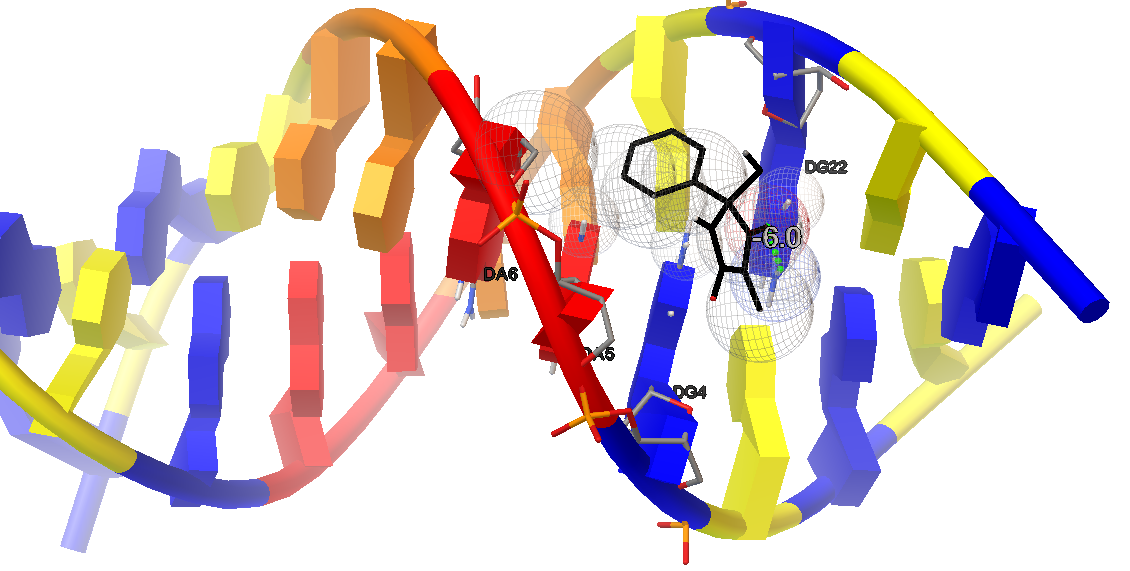
\includegraphics[width=0.8\linewidth]{mephenytoin_ribbon_9.png}
			\caption{\centering The hydrogen bonding interaction \linebreak between Mephenytoin and B-DNA.}
			\label{fig:mph_ribbon}
		\end{figure}
		\vspace{-1.5em}
		\scriptsize
		\begin{table}
			\tiny
			\begin{tabular}{ c | c c c } 
				\multirow{2}{7.6em}{\centering \textbf{Close interactions with B-DNA}}&\multicolumn{3}{c}{\multirow{2}{10em}{\centering DA5, DA6, DG22, DG4}}\\
				&&&\\
				\hline
				\multirow{6}{7em}{\centering \textbf{Hydrogen bonds (Angstrom Å) with B-DNA}}&\multirow{2}{6em}{\centering \textbf{Donor Atom}}&\multirow{2}{4em}{\centering \textbf{Acceptor Atom}}&\multirow{2}{5em}{\centering \textbf{Bond Length (Å)}}\\
				&&&\\
				\cline{2-4}
				&\multirow{2}{6em}{\centering H21 of DG22 (Chain B)}&\multirow{2}{6em}{\centering O2 of Mephenytoin}&\multirow{2}{2em}{\centering 2.1}\\
				&&&\\
				\cline{2-4}
				&\multirow{2}{6em}{\centering H3 of DG22 (Chain B)}&\multirow{2}{6em}{\centering O2 of Mephenytoin}&\multirow{2}{2em}{\centering 2.3}\\
				&&&\\
			\end{tabular}
			\caption{\centering{The close and hydrogen bonds \linebreak between Mephenytoin and B-DNA.}}
		\end{table}
	\end{column}
	\hspace{-1em}
	\begin{column}{0.55\linewidth}
		\centering
		\scriptsize
		\begin{figure}
			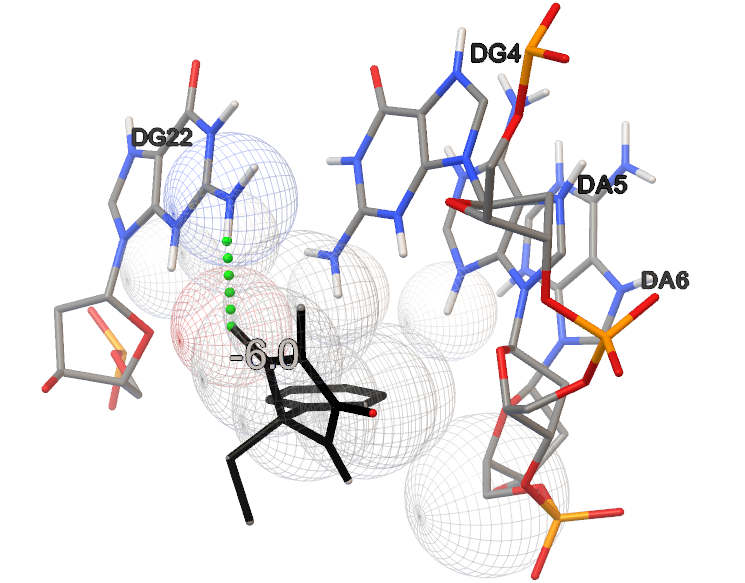
\includegraphics[width=\linewidth]{mephenytoin_yakin_1.png}
			\caption{\centering The close interaction and
				binding affinity \linebreak between Mephenytoin and B-DNA.}
			\label{fig:mph_close}
		\end{figure}
	\end{column}
\end{columns}